\documentclass[a4paper, itemph]{oblivoir}
\setmainhangulfont{NANUMMYEONGJO.TTF}[BoldFont={NANUMMYEONGJOEXTRABOLD.TTF}]
\usepackage[english]{babel}
\usepackage[utf8x]{inputenc}
\usepackage[T1]{fontenc}
%% Sets page size and margins
\usepackage[a4paper,top=3cm,bottom=2cm,left=3cm,right=3cm,marginparwidth=2cm]{geometry}

\usepackage{indentfirst}

%% Useful packages
\usepackage{amsfonts}
\usepackage{amsmath, mathtools}
\usepackage{graphicx}
\usepackage{subcaption}
\usepackage[colorinlistoftodos]{todonotes}
\usepackage{amssymb}
\usepackage{amsthm}
\usepackage{tikz}

%Extravaganza
\newtheorem{thm}{Theorem}[subsection]
\newtheorem{lem}{Lemma}[subsection]
\newtheorem{cor}{Corollary}[subsection]
\newcommand{\overbar}[1]{\mkern 1.5mu\overline{\mkern-1.5mu#1\mkern-1.5mu}\mkern 1.5mu}
\theoremstyle{definition}
\newtheorem{defn}{Definition}[subsection]
\newtheorem{rem}{Remark}[subsection]

\begin{document}
\title{기초전자회로 및 실험: Lab \#05}
\author{서울대학교 전기$\cdot$정보공학부 2018-12602 이준협}
\maketitle

\section{Preliminaries}
This section serves as a short summary to the model of the drain current that this experiment tried to verify. The model includes velocity saturation, the body effect($V_{TH}=V_{TH,0}+\rho(\sqrt{|V_{SB}|+2|\phi_F|}-\sqrt{2|\phi_F|})$), and channel length modulation to explain the drain current. The theory behind the equations are mainly from \textit{Physics of Semiconductor Devices}.

When $V_{SB}=0[V]$, one can express the drain current, with velocity saturation, as
\[I_D=W|Q(y)|v(y)=WC_{ox}(V_{GS}-V_{TH}-V(y)-\rho(\sqrt{V(y)+2\phi_F}-\sqrt{2\phi_F}))\frac{\mu_n E(y)}{1+\dfrac{\mu_n E(y)}{v_{sat}}}\]
when $V(y)$ is the voltage relative to the source. Now, when we linearize $\rho(\sqrt{V+2\phi_F}-\sqrt{2\phi_F})$,
\[I_D(1+\frac{\mu_n E(y)}{v_{sat}})dy=WC_{ox}\mu_n(V_{GS}-V_{TH}-MV(y))E(y)dy \:(M\approx 1+\frac{1}{2}\frac{\rho}{\sqrt{2\phi_F}})\]
when $M$ accounts for the linear approximation of $\rho(\sqrt{V+2\phi_F}-\sqrt{2\phi_F})$($=\dfrac{\rho}{\sqrt{V+2\phi_F}+\sqrt{2\phi_F}}V $$\approx \dfrac{1}{2}\dfrac{\rho}{\sqrt{2\phi_F}}V$). Finally, integrating this equation from $y=0$ to $y=L$ leads to the triode region current
\begin{equation}I_D=\dfrac{WC_{ox}\mu_nE_{sat}}{LE_{sat}+V_{DS}}(V_{GS}-V_{TH}-\frac{MV_{DS}}{2})V_{DS}\:(E_{sat}:=\frac{v_{sat}}{\mu_n})\end{equation}
The saturation voltage can be obtained from determining the voltage when $I_D$ flattens out, i.e. when the tangent slope is zero. The saturation voltage and current can be expressed as
\begin{equation}V_{sat}=\frac{2}{M}\frac{V_{GS}-V_{TH}}{1+\sqrt{1+\dfrac{2(V_{GS}-V_{TH})}{MLE_{sat}}}},\:I_{sat}=\frac{1}{2}\frac{W}{L}C_{ox}\mu_nMV_{sat}^2\end{equation}. Note that the body effect can be incorporated simply by replacing $2\phi_F$ with $2\phi_F+V_{SB}$.

To account for the channel length modulation due to the depletion region at the drain, we can write $L=L_0(1-a\sqrt{1+bV_{DS}})$($\because\sqrt{\dfrac{2\varepsilon_s}{qN_A}(\psi_{bi}-\psi_s+V_{DB})}$ is the depletion width), and linearize $\dfrac{1}{L}=\dfrac{1}{L_0(1-a\sqrt{1+bV_{DS}})}$ as $\dfrac{1}{L'}(1+\lambda V_{DS})$. Note that $-\dfrac{1}{\lambda}$ is the $x$-intercept of the tangent line of $\dfrac{1}{1-a\sqrt{1+bV_{DS}}}$ at the bias point, so $\lambda=\dfrac{ab}{-3aX^2+2X+a}\:(X:=\sqrt{1+bV_{DS}})$. Therefore, we expect $\lambda$ to decrease as $V_{DS}$ increase when $X<\dfrac{1}{3a}\Leftrightarrow V_{DS}<\dfrac{1}{b}\left(\dfrac{1}{9a^2}-1\right)$, which is nearly always the case since $a=\dfrac{1}{L_0}\sqrt{\dfrac{2\varepsilon_s}{qN_A}(\psi_{bi}-\psi_s+V_{SB})}$ is small due to high body doping [1].

\section{$I_D-V_{GS}$ Characteristic Plots}
\begin{figure}[htb]
    \centering
    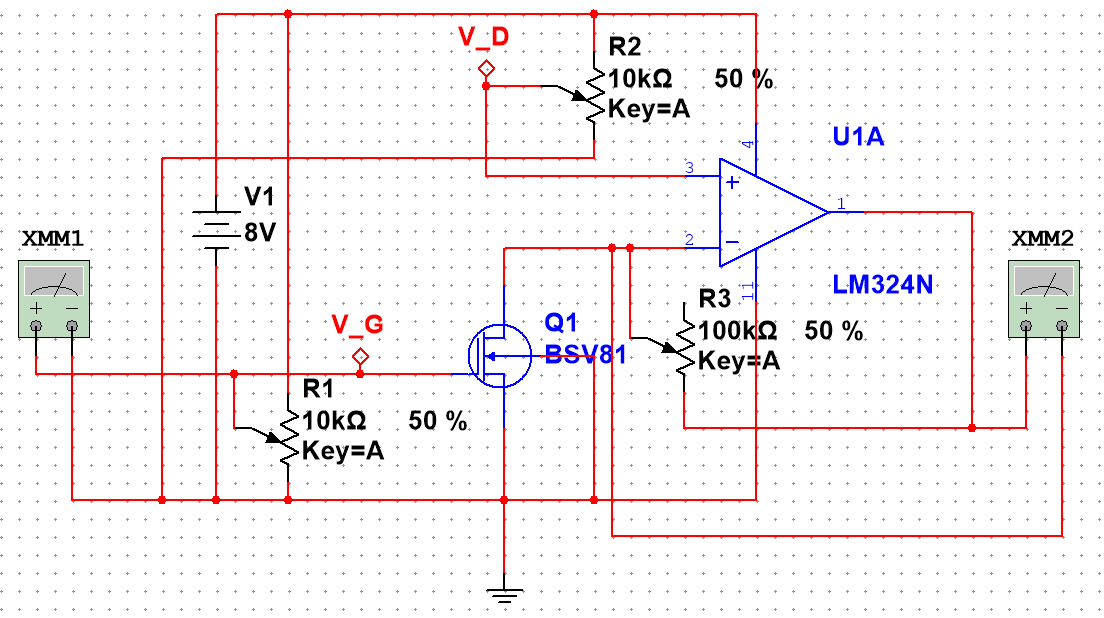
\includegraphics[width=0.465\linewidth]{MOSFET_circuit.PNG}
    \caption{Circuit to measure the $I_D-V_{GS}$ plot. Since the multimeter cannot measure currents in the $\mu A$ range, the current is measured by measuring the voltage across the $100[k\Omega]$ resistor. The op-amp is needed to maintain the drain voltage constant regardless of the current across the $100[k\Omega]$.}
\end{figure}
\begin{figure}[htb]
    \centering
    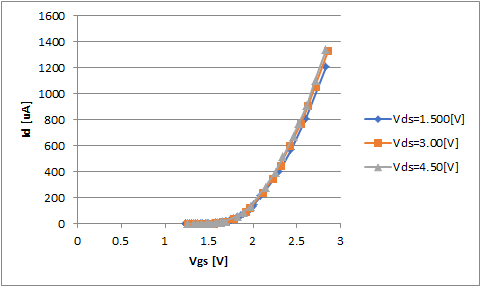
\includegraphics{Vgs-Id_nmos.png}
    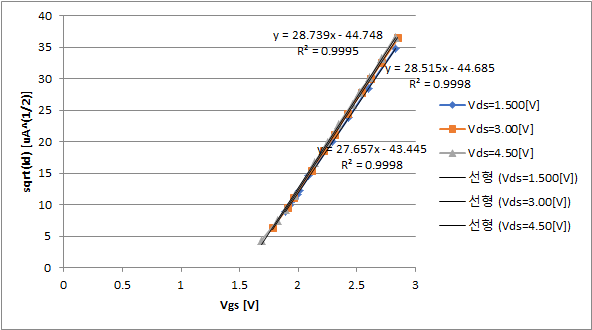
\includegraphics[width=0.465\linewidth]{Vgs-sqrt(Id)_nmos.png}
    \caption{$I_D-V_{GS}$ and $\sqrt{I_D}-V_{GS}$ plots of NMOS \#2 of the HEF4007UBP.}
\end{figure}
\begin{figure}[htb]
    \centering
    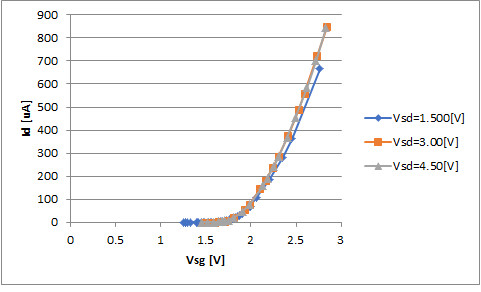
\includegraphics{Vsg-Id_pmos.png}
    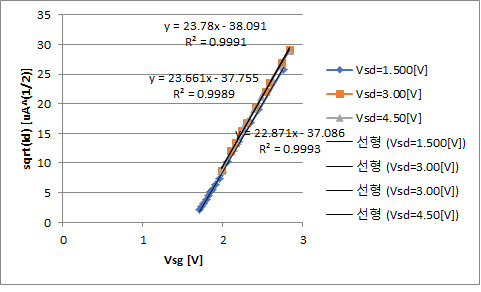
\includegraphics[width=0.43\linewidth]{Vsg-sqrt(Id)_pmos.png}
    \caption{$I_D-V_{SG}$ and $\sqrt{I_D}-V_{SG}$ plots of PMOS \#2 of the HEF4007UBP.}
\end{figure}
The graph of $I_D$ relative to the gate voltage increases superlinearly in both the NMOS and PMOS. The general trend can be viewed as quadratic, which can be seen both in Figure 2 and 3. That is, $1+\sqrt{1+\dfrac{2(V_{GS}-V_{TH})}{MLE_{sat}}}$ can be viewed approximately as a constant near 2. Then equation (2) becomes: $V_{sat}\approx\dfrac{V_{GS}-V_{TH}}{M}$, $I_{sat}\approx\dfrac{1}{2M}\mu_nC_{ox}\dfrac{W}{L}(V_{GS}-V_{TH})^2$. Now, the threshold voltage can be approximated by plotting the $x$-intercept of the linear model fitting the $
\sqrt{I_D}-|V_{GS}|$ curve, as $\sqrt{I_{sat}}=\sqrt{\dfrac{1}{2M}\mu_nC_{ox}\dfrac{W}{L}}(V_{GS}-V_{TH})$.
\begin{table}[htb]
    \centering
    \begin{tabular}{c|c|c|c|c|c|c}
        $V_{DS}[V]$ & 1.500 & 3.00 & 4.50 & -1.500 & -3.00 & -4.50\\
        \hline
        $|V_{TH}|[V]$ & 1.571 & 1.567 & 1.557 & 1.622 & 1.596 & 1.602
    \end{tabular}
    \caption{$V_{DS}-|V_{TH}|$ characteristic. $V_{DS} <0$ stands for the PMOS.}
\end{table}
Although there are errors due to the measurements of the resistance(1\%) and due to the effects of $E_{sat}$, the threshold voltage is measured to be generally decreasing as drain voltage increases, as can be seen in table 1. This is because charge sharing from the drain reduces the burden of the gate to balance out the depletion charge and therefore lowers the threshold voltage [1]. We use $V_{THN}=1.57[V]$ and $V_{THP}=-1.61[V]$, the mean.
\section{$I_D-V_{DS}$ Characteristic Plots}
\begin{figure}[htb]
    \centering
    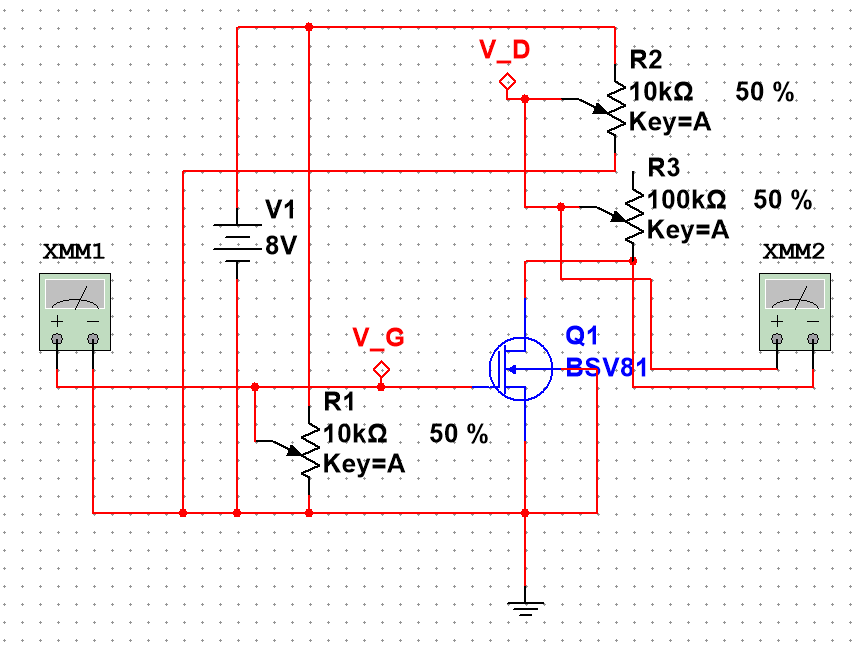
\includegraphics[width=0.4\linewidth]{MOSFET_cir_noamp.PNG}
    \caption{Circuit to measure the $I_D-V_{DS}$ characteristics. The op-amp is omitted since gate voltage is maintained since no current flows into the gate.}
\end{figure}
\begin{figure}[htb]
    \centering
    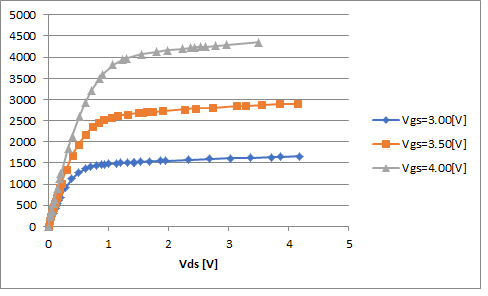
\includegraphics[width=0.4\linewidth]{Vds-Id_nmos.png}
    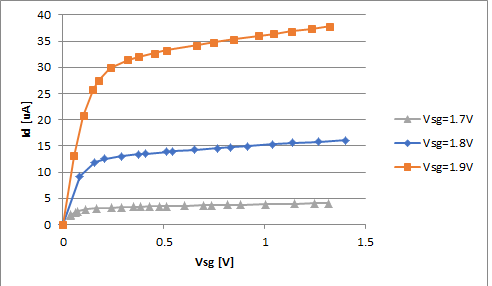
\includegraphics[width=0.41\linewidth]{Vsd-Id_pmos.png}
    \caption{$I_D-|V_{DS}|$ characteristic curves of the NMOS \#2 and PMOS \#2.}
\end{figure}
\begin{figure}[htb]
    \centering
    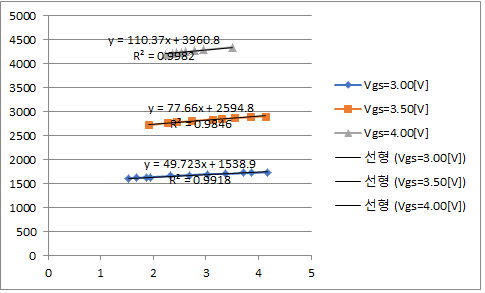
\includegraphics[width=0.4\linewidth]{lambda_nmos.png}
    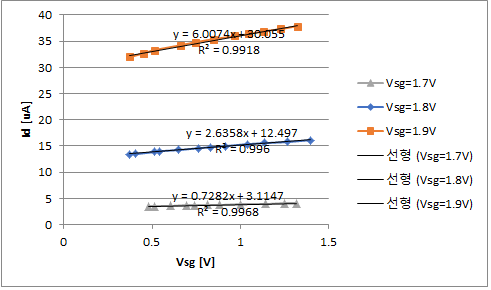
\includegraphics[width=0.4\linewidth]{lambda_pmos.png}
    \caption{Linear fit of the current in the saturation region to determine $\lambda$.}
\end{figure}
The saturation voltage is approximately calculated from calculating the difference between the measured values and the linear model. $V_{sat}=0.7[V]/1[V]/1.3[V]$ in the NMOS, so $M=2.04/1.93/1.87$ when we calculate $\dfrac{V_{GS}-1.57}{V_{sat}}$. $M$ decreases when $V_{DS}$ increases, so this fits in with theory($\because M\approx1+\dfrac{\rho}{\sqrt{V+2\phi_F}+\sqrt{2\phi_F}}$).

$-1/\lambda$ is the $x-$intercept of the linear model in figure 6, and $1/r_o$ is the slope of the linear model($\because I_D=I_{sat}(1+\lambda V_{DS})$, so the $x-$ intercept is $-1/\lambda$, and $\dfrac{1}{r_o}=\dfrac{\partial I_D}{\partial V_{DS}}=I_{sat}\lambda=$(slope)). The results are summarized in table 2. One can see that $\lambda$ decreases as $|V_{DS}|=|V_{sat}|$ increases, as expected by the model.
\begin{table}[htb]
    \centering
    \begin{tabular}{c|c|c|c|c|c|c}
        $V_{GS}[V]$ & 1.500 & 3.00 & 4.50 & -1.700 & -1.800 & -1.900\\
        \hline
        $1/\lambda$[V] & 30.95 & 33.41 & 35.89 & 4.85 & 4.74 & 5.00\\
        \hline
        $\lambda$[$V^{-1}$] & 0.032 & 0.030 & 0.028 & 0.206 & 0.211 & 0.200\\
        \hline
        $r_o$[$k\Omega$] & 20.11 & 12.88 & 9.06 & 1576.29 & 379.39 & 166.46
    \end{tabular}
    \caption{Parameters explaining the channel length modulation effect.}
\end{table}

The mobility parameter $\dfrac{W}{L}\mu C_{ox}$($\mu_n$ for NMOS, $\mu_p$ for PMOS) can be extracted from looking at the linear region. In equation (1), when $V_{DS} \ll 1$, $I_D\approx \dfrac{WC_{ox}\mu E_{sat}}{LE_{sat}}(|V_{GS}|-|V_{TH}|)|V_{DS}|=\dfrac{WC_{ox}\mu}{L}(|V_{GS}|-|V_{TH}|)|V_{DS}|=\dfrac{|V_{DS}|}{R_{on}}$. Since we know $V_{TH}$, we can obtain the mobility parameter from $\dfrac{1}{R_{on}(|V_{GS}|-|V_{TH}|)}$. The results are summarized in table 3. One can see that the parameter decreases as the gate voltage $V_{GS}$ increases. This is because the transverse electric field increases as the gate voltage increases, which pulls electrons more strongly towards the gate, causing more scattering, which leads to a decrease in effective mobility. Also, one can see that the mobility parameter is smaller in the PMOS than in the NMOS, as $\mu_p < \mu_n$.
\begin{figure}[htb]
    \centering
    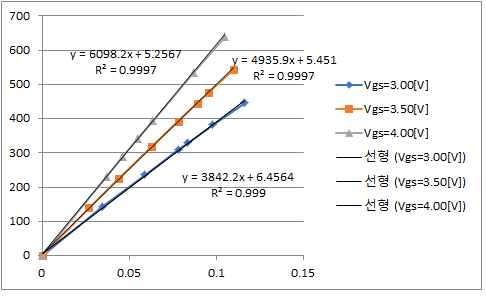
\includegraphics[width=0.4\linewidth]{Ron_nmos.png}
    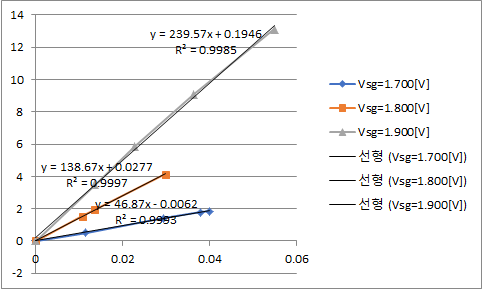
\includegraphics[width=0.4\linewidth]{Ron_pmos.png}
    \caption{Linear fit of the current in the linear region to determine $\dfrac{W}{L}\mu C_{ox}$}
\end{figure}
\begin{table}[htb]
    \centering
    \begin{tabular}{c|c|c|c|c|c|c}
        $V_{GS}$[V] & 1.500 & 3.00 & 4.50 & -1.700 & -1.800 & -1.900 \\
        \hline
        $W\mu C_{ox}/L$[$\mu A/V^2$] & 2686.853 & 2557.461 & 2509.547 & 520.7778 & 729.8421 & 826.1034
    \end{tabular}
    \caption{Effective mobility decrease due to the transverse electric field.}
\end{table}
\section{$V_{TH}-V_{SB}$ Characteristic Plot}
\begin{figure}[htb]
    \centering
    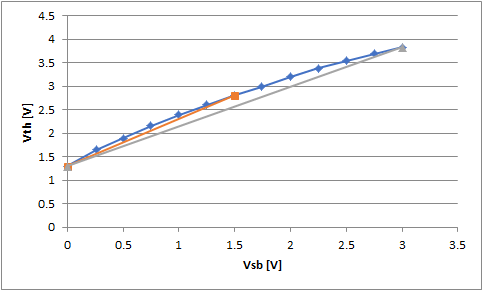
\includegraphics[width=0.5\linewidth]{Vsb-Vth.png}
    \caption{$V_{SB}-V_{TH}$ plot. The slope of the orange line is the rate of change from $V_{SB}=0[V]$ to $1.500[V]$, and the slope of the gray line is the rate of change from $V_{SB}=0[V]$ to $3.00[V]$. The decrease in slope shows the square-root dependence of threshold voltage on $V_{SB}$.}
\end{figure}

The $V_{SB}$ was measured by fixing the base voltage to ground and applying a constant voltage to the source by a voltage follower. The $V_{TH}$ was obtained by measuring the $V_{GB}$ value when $I_{D}$ becomes $0.1[\mu A]$ as to quickly measure multiple threshold voltages (the constant-current method in [2]) and then calculating $V_{TH}=V_{GS}=V_{GB}-V_{SB}$. Now, since $V_{TH}=V_{TH,0}+\rho(\sqrt{2\phi_F + V_{SB}}-\sqrt{2\phi_F})$, we find out $\rho$ and $\phi_F$ from the slope of the orange line and the gray line in figure 6. The slope is $\dfrac{V_{TH}-V_{TH,0}}{V_{SB}}=\dfrac{\rho}{\sqrt{2\phi_F + V_{SB}}+\sqrt{2\phi_F}}$, so the slope of the orange line is $\dfrac{\rho}{\sqrt{2\phi_F + 1.500}+\sqrt{2\phi_F}}$ and the slope of the orange line is $\dfrac{\rho}{\sqrt{2\phi_F + 3.00}+\sqrt{2\phi_F}}$. $\phi_F$ can be found out by finding out the appropriate value to $\phi_F$ when the ratio of the two slopes, $\dfrac{\sqrt{2\phi_F + 1.500}+\sqrt{2\phi_F}}{\sqrt{2\phi_F + 3.00}+\sqrt{2\phi_F}}$, becomes the measured value. We calculate $\phi_F=336.9[mV]$. Now, $\rho=2.306[V^{1/2}]$ can be calculated from plugging in $\phi_F$. We verify this measurement by calculating $M\approx 1+\dfrac{1}{2}\dfrac{\rho}{\sqrt{2\phi_F}}=2.405$ and comparing this with the measured $M$ calculated in section 2 by $\dfrac{V_{GS}-V_{TH}}{V_{sat}}=2.04/1.93/1.87$. Since $2.405$ is of the same order with the measured values and since it is larger than all of the values, we can assume that the measurements agree with theory.
\section{Overview}
\begin{figure}[htb]
    \centering
    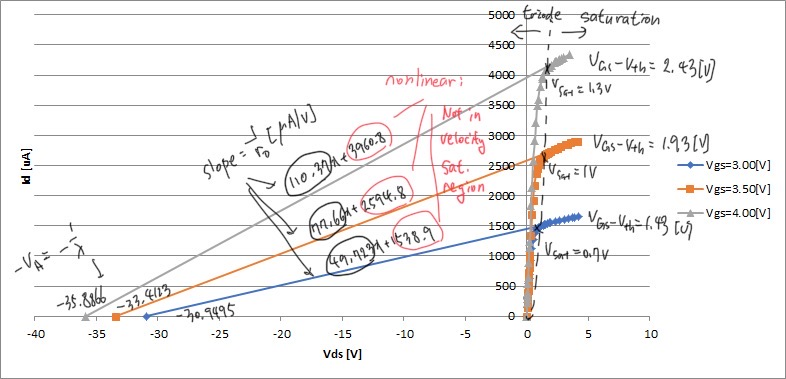
\includegraphics[width=0.9\linewidth]{overview.JPG}
    \caption{Overview of the parameters of the NMOS measured in lab 5.}
\end{figure}
Since the resistance of the variable resistors kept changing due to mechanical vibrations in the circuit, some measurements seemed as if it didn't conform to theory($V_{TH}$ didn't change much according to $V_{DS}$, so even 1\% of error is not tolerated). Nonetheless, the model including $M$ and $\lambda$ was well confirmed by this experiment. Also, the difference in mobility followed the trend of effective mobility when gate voltage is changed, as predicted in [1].
\begin{thebibliography}{}

\bibitem{1} S. M. Sze and K. K. Ng, \textit{Physics of Semiconductor Devices}, 4th ed. Hoboken, NJ: Wiley, 2015, pp. 293-338.
\bibitem{2} A. Ortiz-Conde et al., “A review of recent MOSFET threshold voltage extraction methods,” \textit{Solid-State Electron.}, vol. 47, no. 4, pp. 677–683, 2003.
\end{thebibliography}

\end{document}
